\chapter{Appendix - 1}

\section*{Nādānusandhāna --- An Overview of the Haṭhayogic practice}

\centerline{\textbf{Dr.~Jayaraman Mahadevan}}

\section*{Introduction}

This article endeavors to present a general overview of a Yogic practice called Nādānusandhāna based on the text Haṭhayogapradīpikā of Svātmārāma with inputs from Jyotsnā commentary on the text by Brahmānanda. In the process, a brief relevant reference on the theme from Yogasūtra-s is also presented.

\section*{What is Nāda?}

Nāda is defined as (Vācaspatya\footnote{Vacaspatyam is a Sanskrit Lexicon, of 5442 pages, by Pandit Taranatha Tarkavacaspati (1812-1885), Calcutta that that takes into account the entire spectrum of Sanskrit literature in explaining any given Sanskrit term.} pg.~4030)

\begin{shloka}
nābherūrdhvaṃ hṛdi sthānāt mārutaḥ prāṇasaṃjñakaḥ|\\
Nādati brahmarandhrante tena nādaḥ prakīrttitaḥ||
\end{shloka}

\begin{quote}
\textit{Above the Navel, from the place of the heart, till Brahma-randhra (Suture or aperture in the crown of the head) Prāṇa resonates. This resonation of Prāṇa is called as Nāda.}
\end{quote}

\begin{shloka}
ākāśāgnimarujjāto nābherūrddhvaṃ samuccaran |\\
mukhe'tivyaktamāyāti yaḥ sa nāda itīritaḥ ||
\end{shloka}

\begin{quote}
\textit{That which takes birth by the combination of Ākāśa (ether), Fire (Agni) and  Marut (Air) and moves above the navel and is intensely manifest in the mouth is called as Nāda.}
\end{quote}

Going by the above definition it can be seen that Nāda is Prāṇa and its reverberation that finds special manifestation through the organ of speech. 
  
\section*{Nādānusandhāna in the Yogasūtras?}

Though the term Nāda is not directly found on the Yogasūtras there is a very important discussion on Praṇava. Praṇava is regarded as the primordial sound cutting across disciplines of ancient origins in India which is evidenced by the following Puranic reference -

\begin{shloka}
oṅkāraścātha śabdaśca dvāvetau brahmaṇaḥ purā |\\
kaṇṭhaṃ bhittvā viniryātau tasmānmāṅgalyakāvimau ||\\
\versenum{Bṛhan-nāradīya-purāṇa (1.51.10)}
\end{shloka}

\textit{Praṇava and the word Atha are the two first sounds that emerged from the throat of the creator and hence both are considered very auspicious.}

In Yogasūtra 1.27 Sage Patañjali states that Īśvara is indicated by the term Praṇava. The following commentary to this Sūtra by Svami Vivekananda brings out the significance of Praṇava Nāda– 

\begin{quote}
\textit{“In making a sound we use the larynx and the palate as a sounding board. Is there any material sound of which all other sounds must be manifestations, one which is the most natural sound? Om (Aum) is such a sound, the basis of all sounds. The first letter, A, is the root sound, the key, pronounced without touching any part of the tongue or palate; M represents the last sound in the series, being produced by the closed lips, and the U rolls from the very root to the end of the sounding board of the mouth. Thus, Om represents the whole phenomena of sound-producing. As such, it must be the natural symbol, the matrix of all the various sounds. It denotes the whole range and possibility of all the words that can be made.”}
\quoteauthor{(Raja Yoga pg.127-128)}
\end{quote}

Further Sūtra 1.28 presents the utilization of this Praṇava-nāda. It states that Praṇava has to be repeated along with the reflection on the meaning it indicates i.e Īśvara. This can considered as the discussion on Nāda and its utilization in meditative purposes (anusandhāna)  in the Yogasūtras, the principal text of Yoga.

\section*{Nādānusandhāna in Haṭhayoga tradition}

Originally, the term Nādānusandhāna is found in the Haṭhayoga texts that come after the Yogasūtras of Patañjali. Though there are many texts in Haṭhayoga tradition, Haṭhayogapradīpikā, a 15th CE text by Svātmārāma is considered one of the finest works in this field. It is studied widely to understand the fundamentals of Haṭhayoga.

Svātmārāma the author of Haṭhayogapradīpikā states that there are four limbs of Haṭhayoga (1.56) –

\begin{shloka}
āsanaṃ kumbhakaṃ citraṃ mudrākhyaṃ karaṇaṃ tathā|\\
atha nādānusandhānamabhyāsānukramo haṭhe||
\end{shloka}

\begin{quote}
\textit{Āsanas, Various kinds of Kumbhakas (Prāṇāyāma), the finest tool called Mudrā and the Nādānusandhāna. It is in this sequence, the practice of Haṭha should be done.}
\end{quote}

As can be seen in the verse above, Nādānusandhāna has been listed as the final limb of Haṭha that comes after a good level of mastery in \textit{Āsana}, \textit{Prāṇāyāma} and \textit{Mudrās}. It is to be noted that the chapterization of the Haṭhayogapradīpikā is also based on this sequence of the tools of Haṭha. Hence Nādānusandhāna in discussed in the fourth Upadeśa (chapter) of the text.   

\section*{Nādānusandhāna ---  Its definition and its practice:}

The fourth Upadeśa (chapter) of Haṭhayogapradīpikā beings (4.1) with a salutation to Lord Śiva who is also the called as Ādinātha or the first teacher in the tradition of the Nāthayogins, This verse of salutation incorporates the term Nāda - 

\begin{center}
namaḥ śivāya gurave nādabindukalātmane\\
\textit{Salutations to lord Śiva who embodies Nāda, Bindu and Kala.}
\end{center}

It is worth noting that Nāda in this context is defined in the Jyotsanā commentary to Haṭhayogapradīpikā as –

\begin{quote}
\begin{center}
\textit{kāṃsya-ghaṇṭā-nirhrādavad anuraṇanaṃ nādaḥ Nāda refers to the reverberation (inside the body) that is similar to that of the reverberating bronze bell.}
\end{center}
\end{quote}

\section*{Importance of Nāda in Yoga}

At the very outset, the importance of Nāda in achieving the yogi goal of focus of the mind is established by the following verse (4.29)-

\begin{shloka}
indriyāṇāṃ mano nātho mano nāthasyatu mārutaḥ\\
mārutasya layo nāthaḥ sa layo nādamāśritaḥ||
\end{shloka}

\begin{quote}
\textit{The senses are controlled by the mind. The mind is controlled by the breath. Absolute control over the breath happens when the mind gets dissolved. The dissolution or absorption of the mind is based on Nāda}
\end{quote}

\section*{Who is Eligible of Nādānusandhāna?}

Before proceeding further, Svātmārāma clarifies as to whom is the practice meant for? He states (4.65)-

\begin{shloka}
aśakyatattvabodhānāṃ mūḍhānāmapi sammatam|\\
proktaṃ gorakṣanāthena nādopāsanamucyate|| 
\end{shloka}

\begin{quote}
\textit{Nādānusandhāna, a practice that has been prescribed by Gorakṣanātha, is agreeable and accessible even to those who are not intellectually capable of grasping subtle principles.}
\end{quote}

Thus it becomes evident that a meditation that is based on the Nāda is equally applicable to entire range of Sādhakas –Manda (the beginner), Madhyama (intermediate) and Uttama (the advanced).

\section*{Two methods of Practice of Nādānusandhāna}

\subsection*{Method 1}

The first method of Nādānusandhāna is found from verse 67 to 81 of the fourth Chapter of Haṭhayogapradīpikā. The general Purport of first method of Nādanusandhāna is presented below.

Being seated in Mukt\textit{Āsana} a Yogi should practice either the Śaṇmukhī-mudrā or the Śāmbhavaī-mudrā and should attain one pointed focus of the mind. With this focus one should now turn his attention on the Nāda in the Suṣumnā that has been cleansed of its impurities by Various \textit{Prāṇāyāma} practices. (4.67,68)

There are four stages in this practice (4.69-77). They are

\begin{enumerate}
\itemsep=0pt
\renewcommand{\theenumi}{\alph{enumi}}
\renewcommand{\labelenumi}{\theenumi.}
\item Ārambha 
\item Ghaṭa
\item Paricaya
\item Niṣpatti 
\end{enumerate}

In the Ārambha stage --- when the Prāṇa after entering the Suṣumnā reaches the Anāhata-cakra– which is variously indicated as the space of \textbf{the heart --- solar plexus}, a Nāda that generates bliss is heard. \textbf{It resembles the tinkling of various jewels.} When the practitioner focuses on this sound he becomes blissful, becomes free from disease, his/her heart is full of Prāṇa, divine fragrance emanates from him/her and he/she shines with lusture. 

In the Ghaṭa Stage --- The Prāṇa raises from the heart to \textbf{the throat region} --- the region of Viśuddhi-cakra. The Nāda that emerges resembles the sound of the \textbf{rumbling sound of the kettle drum} --- bheri.

In the Paricaya stage --- the Prāṇa now raises further and reaches the \textbf{place in between the eye brows} which is ājñā-cakra.  Then sounds of the drum called Mardala is heard here. This is the place of all siddhis --- divine powers. This also delivers a Yogi from pain, old age, disease, hunger and somnolence.
 
In the fourth and final stage of Niṣpatti --- the Prāṇa raises and reaches the \textbf{aperture in the skull} which is called as the Brahmarandhra and here the \textbf{sounds of Vīṇā - the lute and Veṇu --- the flute} are heard. 

Thus the movement of Prāṇa in these four stages in the Suṣumnā Nāḍī leads to the total absorption --- laya --- this bestows bliss that is unsurpassable. Svātmārāma even states “let there be liberation or not, here is perfect bliss” (4.78). Further he states, In the hearts of Great Yogin-s who remain in a state of Samādhi through concentration on Nāda, there is a plentitude of bliss, unequalled surpassing all description and which the blessed teacher alone knows (4.81). 

\begin{figure}
\centering
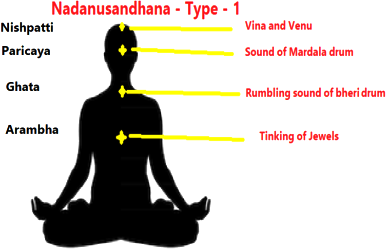
\includegraphics[scale=.8]{images/fig1.png}
\end{figure}

\section*{Method 2 of Nādānusandhāna}

The second method of Nādānusandhāna is described from verses 4.82 to 89 of Haṭhayogapradīpikā. The Purport of the practice is given below.

With the thumbs one should close one’s ears and focus the mind on the Nāda – the inner sound. Through this process of sustained hearing, the inner sound drowns the external sound. By this Yogi overcomes all distractions and becomes happy (4.82)

During the initial stages various prominent sounds are heard but when progress is made more and more subtle sounds are heard. (4.) 

\subsection*{In the beginning}

 various sounds resembling those of \textbf{the ocean, the cloud, the kettle drum and the jarjhara (tabor) drum} is heard. \textbf{In the middle}, sounds that resemble \textbf{the drum, the conch, the bell and the horn} are heard. \textbf{Finally}, the sounds that resemble those of \textbf{tinkling bells, the flute, the Vīṇā and the bees} are heard. (4.85,86) 

Certain guidelines in this practice are to be followed (4.87 -- 89) -

\begin{enumerate}
\itemsep=0pt
\item In case of coexistence of greater and subtler inner sounds one should allow the mind to focus only on the subtler sounds. 
\item Even though attention may shift from the gross to the subtle sounds or the vice versa, the mind should stay with the Nāda and should not be allowed to drift away elsewhere.
\item In whatever inner Nāda the mind gets focused, gets steadiness, that is the path way for the mind to get dissolved. 
\end{enumerate}

\section*{How Nādānusandhāna Captivates the mind}

A series of beautiful examples are provide to illustrate how Nāda captivates the mind and makes it focused (4.90--97): -

\begin{enumerate}
\itemsep=0pt
\item As the \textbf{bee drinking honey} care not for the fragrance, so the mind absorbed in Nāda does not crave for objects outside.
\item Nāda is like the sharp goad that curbs the volatile action of the \textbf{elephant in rut} called the Mind.
\item Nāda makes the mind totally immobile, like the \textbf{bird that has lost its wings.}
\item Nāda is like the net that captures the \textbf{restless deer} called the mind.
\item Nāda is also like the hunter who kills \textbf{the deer} called the mind --- this refers to the state of transcending the mind. 
\item Nāda is also like the bolt that locks down the \textbf{horse} called the mind and channelizes its movement. 
\item Nāda makes the mind motionless like \textbf{the serpent} that is hearing music and it does not run away anywhere.
\end{enumerate}

\section*{Nādanusandha --- the final steps}

The dissolution of the mind taking that was absorbed into Nāda is detailed in the final set of Verses on Nādānusandhāna (4.98-102) 
 
It states that the fire burning in a piece of wood, subsides along with the burnt wood. So also the mind directed to Nāda is absorbed along with it. In essence it means, Rajas and Tamas are absorbed by Nāda which is Sāttvika. And with intensification of the practice of Nādānusandhāna and Vairāgya, in due course, even this Sāttvika activity also dies down and the mind also dissolves into its cause. (4.98)

Further, the text observes, the inner Nāda stems from the self-luminous consciousness. The mind that focuses on the Nāda gradually gets absorbed into the light and that is the eternal abode of Lord Viṣṇu. (4.100) This is indeed an unique idea – Sound merging into light.
 
Finally the texts states that Nāda is the Shakti of the Paramātman and when once the mind takes recourse to this Shakti and gets absorbed all that remains is Silence and that is the establishment of the Consciousness in its true nature (4.101-102).  

%~ \begin{center}
%~ \textbf{Select References}
%~ \end{center}

\begin{thebibliography}{9}
\bibitem{1} Tarkavachaspati, Sri Taranatha (1962), Vacaspatya, Chowkhamba Saṃskṛta Series, Varanasi, 
\bibitem{2} Haṭhayogapradīpikā of svātmārāma with the commentary jyotsnā  of Brahmānanda, (1972)The Adyar Library and Research Center, Madras 
\bibitem{3} Vivekananda, Swami,  (1920), Rājayoga, Weed-parsons Printing company, New York (pdf of the book accessed from the web: \url{https://archive.org/details/RājayogaSwamiVivekananda1920})
\end{thebibliography}
